\documentclass[fleqn,12pt]{article}

\usepackage{setspace,url,fullpage,latexsym,amsmath,amsthm,amssymb,pifont,graphicx,appendix,float,rotating,caption,subcaption,multirow,longtable,colortbl,natbib,graphics,graphicx,enumitem,pdflscape,epstopdf,verbatim,longtable}

\setcitestyle{aysep={},yysep={;}}
\bibliographystyle{apsr}


\usepackage{lipsum}
\usepackage{filecontents}
\usepackage[dvipsnames]{xcolor}
\usepackage{hyperref}
\usepackage[utf8]{inputenc}
\usepackage{cleveref}
\usepackage{pdflscape}
\usepackage{afterpage}
\usepackage{capt-of}
\usepackage{soul}
\hypersetup{
	backref =       true,
	pagebackref  =  true,
	colorlinks =    true,
	linkcolor =     blue,
	anchorcolor =   [rgb]{0.0,0.9,0.9},
	citecolor =     blue,
	filecolor =     [rgb]{0.0,0.1,0.7},
	urlcolor =      [rgb]{0.0,0.0,0.7},
}

% Packages for regression table
\usepackage{booktabs}
\usepackage{siunitx}
\newcolumntype{d}{S[
    input-open-uncertainty=,
    input-close-uncertainty=,
    parse-numbers = false,
    table-align-text-pre=false,
    table-align-text-post=false
 ]}

\doublespacing

\title{\singlespacing A Wiki-based Dataset of Military Operations with Novel Strategic Technologies (MONSTr)}
\author{Authorship Anonymized}
\vspace{.1cm}
\date{}

\usepackage{helvet}
\usepackage{titlesec}
\graphicspath{{./figures/}}

\titleformat{\subsubsection}
{\normalfont\fontsize{12}{17}\bfseries\slshape}
{\thesubsection}
{1em}
{}

\begin{document}
	\maketitle
	\thispagestyle{empty}
	\setcounter{page}{0}
	
	\begin{abstract}
            \singlespacing \noindent Research on strategies and force structures in modern warfare is prolific, but siloed. While some examine boots on the ground, others focus on aerial bombing or unpiloted platforms. Consequently, most studies focus on the effects of one approach, seldom considering it in lieu of or conjunction with others. Furthermore, there is less knowledge on the origins and implementations of these strategic choices analyzed in isolation. The primary reason for these gaps lies with data limitations. This paper introduces a comprehensive dataset on the universe of United States military interventions from 1989-2021 from a single source: Wikipedia. Using automated extraction techniques on its two structured knowledge databases$-$Wikidata and DBpedia$-$we uncover information about nearly every post-1989 military intervention described in existing academic datasets plus 425 additional operations. The data we introduce offers unprecedented coverage and granularity that enables analysis of myriad factors associated with how, when, and where the United States conducts military interventions. We describe the data collection process, demonstrate its contents and validity, and discuss its potential applications to existing theories about force structure design and strategy in war.\\
		\vspace{.1in}
		\noindent
		\textbf{Keywords:} military intervention, use of force, dataset
	\end{abstract}
	
\newpage
\noindent

\section*{Introduction}
Despite being critical of the War on Terror, United States (US) President Obama amplified it upon assuming office and personally ensconced himself in the drone ``kill list" approval chain. Then-Director of National Intelligence Blair explained this pivot: ``It is the politically advantageous thing to do$-$low cost, no US casualties, gives the appearance of toughness” \citep{becker_secretkilllist_2012}. Critics argue that these benefits are outweighed by strategic costs such as backlash, radicalization, and increased terrorist recruitment \citep{kilcullen_opiniondeathoutrage_2009}. Obama's decision was not, however, whether or not to use drones. It was whether to use drones rather than insert or maintain boots on the ground in the ongoing wars in Iraq and Afghanistan that he campaigned on ending. It was whether to use drones rather than manned flights outside of active war theaters.
	
Current research on how states use military force either focuses on the most aggregate level of the war or explains a particular tool in isolation. Consequently, variation in how states design and deploy force structures over a multi-year campaign remains unexplained. So does the relationship between complementary or substitutable types of force. As a result, academic understanding of how states fight is limited, being highly generalized on one side and siloed into individual domains or platforms on the other. There is a sprawling gap between these, where the actual warfighting occurs. Scholars interested in the prosecution of conflict contend with a dearth of data on the means of force across a comprehensive list of military operations. This paper debuts our attempt to overcome it.

We seek to remedy these shortcomings by providing a dataset that captures the means of force across a more expansive universe of US military operations using a familiar, yet under-utilized data source: Wikipedia. Existing datasets focus on higher levels of aggregation like the broader military intervention in part because collecting such information manually is intensive and oft incomplete.\footnote{For instance, \citet[549]{allen_understandingimpactair_2017} remark that ``[i]deally, the unit of analysis for this project would be at the campaign level. Unfortunately, while most modern Western militaries operate in terms of campaigns, data for all countries over time was [sic] not available at the campaign level”.} Aware of the stigma attached to Wikipedia, we nonetheless note that what we gain is worth the tradeoffs. By scraping the Wikiverse for pages on post-1989 US military operations that occurred within the auspices of a US military intervention, our dataset identifies over 300 military operations, most of which existing datasets aggregate into broader wars. Using Wikidata and DBpedia, the structured bedrocks of Wikipedia, we can also extract a host of fine-grained covariates concerning each military operation's dates, belligerents, location, and means used. Since these variables are less subject to human interpretation than those like conflict outcome or objective, concerns about data quality are mitigated (though still addressed). We hope to convince that such a Wiki-based dataset on Military Operations with Novel Strategic Technologies (MONSTr) is not such a monster after all.
	
The paper proceeds with a section on our motivation, in which we trace the mismatch between our research interests and existing theory and data. Next, it outlines our approach in collecting, validating, and organizing the data gleaned from our Wikipedia extraction endeavor. Following this, we describe the dataset's distinctive features to convey the value added, suggesting how scholars might use them to extend or improve studies on how combatants fight. Specifically, we detail its increased breadth and depth, measures of the means of force for each intervention, geographic precision, and thoroughness in identifying the roster of combatants on all sides. The penultimate section presents a data demonstration, predicting the means of military force with theoretically derived determinants drawn from existing scholarship. We conclude with a summary discussion, admission of limitations, and suggestions for future research using the MONSTr dataset.

\section*{Motivation}
A central question in international security concerns how strong states fight, and why. Sometimes they choose losing strategies against weak actors \citep{arreguin-toft_howweakwin_2001}. Military myopia arguments \citep{gentry_doomedfailamerica_2002, lyall_ragemachinesexplaining_2009}, capital-rich force structure narratives \citep{gartzke_democracypreparationwar_2001, caverley_mythmilitarymyopia_2009}, and uncertainty in pre-war estimates of costs and success \citep{sullivan_militaryinterventionpowerful_2009} explain many of these cases. Yet sometimes, despite bureaucratic inertia, economic factor abundance, and the fog of war, advanced militaries deploy ideal force structures against innovative weak enemies. Empirical tests of these theories are limited, however, by inadequate data required for validation. 

We identified three barriers to testing theoretical models of how states fight with existing data. First, we are interested in the planning and execution of military strategy \textit{during} armed conflict \citep{wallace_alliancesinstitutionaldesign_2008}. Most of the research and data has focused on its beginning$-$bargaining, causes, onsets$-$and end$-$duration, outcomes, aftermaths. Notwithstanding the profound knowledge they have yielded, these approaches black box the prosecution of war. This is surprising since we think its conduct has much to tell us about its causes and consequences. Some studies breach the black box of military force to analyze approaches within, but typically focus on the possession of these platforms rather than their use, offering insight only on the latent potential for force.\footnote{Recent exceptions that focus on use include \citet{martinezmachain_aircampaignduration_2015}, \citet{post_flyingfailcostly_2019}, and \citet{gannon_oneifland_2022a}.} Furthermore, the majority bore a peephole onto a single platform or force structure rather than pop open the box. Some look at nuclear platforms \citep{gartzke_determinantsnuclearforce_2014}, naval power \citep{crisher_powerseanaval_2014}, aerial bombing \citep{pape_bombingwinair_1996}, air power more broadly \citep{horowitz_whendoesaerial_2001, martinezmachain_aircampaignduration_2015, allen_understandingimpactair_2017}, ballistic missiles \citep{reiter_ballisticmissilesinternational_2013}, cruise missiles \citep{early_climbingladderexplaining_2022}, or drones \citep{fuhrmann_droningexplainingproliferation_2017}.

This leads to the second barrier$-$siloed scholarship that inhibits the idea of substitutability \citep{morgan_modelforeignpolicy_2000}. At a high level, the substantial foreign policy literature reflects this standpoint by depicting a state's toolkit in broad categories$-$military, diplomatic, economic, cultural, etc. That same logic applies within each category. Leaders craft the use of military force not as isolated dichotomous decisions, but from a menu of substitutable (or complementary) options. Being domain- or platform-specific, existing datasets on the means of force are difficult to harmonize. Rather than peepholes into the blackbox of military force, our research questions on force structure and strategy require it to be open and well-lit. Once again, our inquiries on how and why states fight fall between existing theory and data, generalized on one side, specific but partitioned on the other.

Finally, holding the universe of military interventions and the idea of substitutability in mind, a concern about assumptions of independence across observations crops up. If we seek to explain why an intervention featured solely unpiloted systems, perhaps it is relevant if it is part of a decapitation campaign in enemy territory. Or if a sizable contingent of troops is deployed for a manpower surge in, say, a place like Iraq, perhaps one might expect interventions nested within such a surge campaign to feature a higher frequency of ground troops. Attempting to explain force structure choices outside the strategic contexts in which they occur might lead to bias in estimating independent causal impacts. Yet existing datasets largely list interventions within the same campaign as distinct observations.

\section*{Our Approach}
To surmount these barriers, we produced a dataset that features 1) measures of the means of military force across 2) a comprehensive and more disaggregated list of US military interventions that 3) captures dependence between observations using a consistent unit of analysis. Given the labor-intensive nature of manual data collection, we turned to the structured knowledge graphs of a familiar, underutilized source of information on political events: Wikipedia. There is virtually no scholar who promotes Wikipedia citations, but there is also virtually no scholar who does not queue up a Wiki page for initial information about a topic. While expert knowledge is required to measure contested or complex concepts like conflict outcome or purpose, it is less necessary to identify objective datapoints like the location, participants, and dates of an event. When collected carefully, we contend that the breadth, depth, and granularity of such information easily extracted through automated processes is worth the taboo trade-off.

We disciplined our collection efforts definitionally, in space, and in time to curate a dataset on US military interventions from 1989 to January 2021. Insofar as our case selection is most consistent with the exemplary Military Interventions by Major Powers (MIPS) dataset’s definition, it merits quoting. An intervention is: 

\begin{quote}\singlespacing
``a use of armed force that involves the official deployment of at least 500 regular military personnel (ground, air, or naval) to attain immediate term political objectives through action against a foreign adversary. Routine military movements and operations without a defined target like military training exercises, the routine forward deployment of military troops, non-combatant evacuation operations, and disaster relief should be excluded” \citep[][3]{sullivan_militaryinterventionpowerful_2009}. 
\end{quote}

\noindent \doublespacing
Like MIPS, we exclude threats, training exercises or mobilizations that demonstrate rather than apply force, ebbs and flows of personnel and materiel at permanent military bases, diplomatic cover and evacuation, and humanitarian operations. We deviate from MIPS in that we do not set a size threshold for inclusion.

We also lean on the International Military Intervention (IMI) dataset’s definition, which clarifies that events must be purposeful \citep{pearson_internationalmilitaryintervention_1993, kisangani_internationalmilitaryintervention_2008}. Thus, we omit accidental and unintentional clashes. For instance, if troops deployed along the Iraq border have an unexpected encounter with Syrians, we view it as simply that—a military intervention in Iraq that entailed a contingent clash with Syrians who meddled at the border. Being outside the politically determined mission scope, such a clash (or airspace violation) does not constitute a separate intervention. We also insist that political and military objectives cannot be delinked, disqualifying nonpolitical uses of force. Table \ref{tableA1} in the Appendix summarizes our nearness to MIPS and IMI across definitional fine points, and our departures from the broader approaches of RAND \citep{kavanagh_characteristicssuccessfulmilitary_2019} and Military Intervention Project (MIP) \citep{kushi_introducingmilitaryintervention_2022}. Focusing on definitions of intervention, we omit other important datasets that take a broader approach in this section that we later consider.

Our dataset includes some paramilitary activities. Specifically, we capture some Central Intelligence Agency (CIA) drone strikes, but not all. We defend this on two fronts. First, drones are distinct as a means of force since some are operated by the military (in combat zones) and some by the CIA (in noncombat zones). In fact, extensive criticism has been levied at the CIA program for its lack of military control and transparency. Second, every dataset on military interventions exhibits nonrandom missingness on some drone cases due to their covert nature (even those devoted solely to drone strikes). MONSTr’s coverage is appealing in that the drone strikes it includes have met some threshold of public awareness to make it onto Wikipedia. Since we expect that public constraints amid the domestic politics of war are meaningful factors in how states fight, we accept this bias. In fact, given this variation there should be scholarly pursuits identifying what criteria determines publication on Wikipedia in the first place, a question our dataset allows us to pose and test.

Similar in logic, by nature of being collectible from the internet our cases are open source. There are interesting questions about the deployment of covert force, but we appreciate former Department of Intelligence Director Wilson's comment that ``90\% of intelligence comes from open sources. The other 10\%, the clandestine work, is just the more dramatic. The real intelligence hero is Sherlock Holmes, not James Bond" \citep{lands_publiclyavailableinformation_2019}. It's elementary$-$we leverage the data that are available and focus on research puzzles that interface with public attention and scrutiny.

Next, we spatially confined our sample to cases featuring the United States. Insofar as our impetus to collect these data is to examine how strong states fight, the US is a paragon. Its prolific intervention record also allows us to maximize observations in a pilot probe with one case. The US case is also deeply studied and data rich, better allowing us to test our theories and compare findings. Finally, we temporally confined our scope to start in 1989, when the US first used cruise missiles in conflict. With a special interest in the politics of emerging technologies, we aimed to collect a sample with temporal consistency in the military options, from ground troops to unmanned platforms, available to conflict decision-makers.

Of course, many of these scope limitations can and should be relaxed. Theoretical debates about how states fight would benefit from empirical information concerning pre-1989 interventions, non-US interventions, and a more expansive definition of military force. The dataset presented here is a proof of concept for the validity and value of using Wikipedia to identify and structure such information. Future iterations of the project will expand in precisely these directions. In the following section, we describe the data collection process, with an emphasis on justifying our source, before demonstrating the data's yields and potential.

\section*{Dataset Inputs}
\subsection*{\textit{Collection - Scraping and Patching}}
For most readers, the Wiki interface is familiar. An executive summary sits under the page name, followed by a more detailed description of the entity, event, or concept. Most pages also contain an infobox containing a summary of attributes. For example, the ``cosmic latte" page informs that this is the average hue of the universe based on spectral analysis of over 200,000 galaxies. The sections describe the discovery and naming of the color.\footnote{Thank goodness ``primordial clam chowder" didn't win.} These data, like most other sources available to scholars, are unstructured and require manual review and entry.

Unlike most other sources, Wikipedia rests upon two Resource Description Format (RDF) databases: Wikidata and DBpedia \citep{malyshev_gettingmostout_2018}. Wikidata contains ontology for over 99 million items and their properties as ``triples." Each unique numeric identifier features a structured 1) subject, 2) predicate, and 3) object. For example, Germany (subject) has the capital (predicate) of Berlin (object). DBpedia maps information from each page's infobox also as structured content that can be semantically queried. Since both databases exist in a uniform, machine-readable format, we were able to scrape a comprehensive list of Wikipedia pages describing a US military intervention from 1989 onward using SPARQL, an RDF query language. The resulting data contained over 500 entries and dozens of columns containing structured information from Wikidata and DBpedia infoboxes. After reasonable efforts by research assistants to locate missing data from alternative sources, the neonate MONSTr had few holes.

\subsection*{\textit{Cleaning - Auditing and Validating}}
The primary contribution of our research method also constitutes its greatest burden: justifying Wikipedia itself. It carries a strong stigma in scholarly research that will be difficult to shake \citep{becker_researchfauxpas_2015}.\footnote{Please go read the entertaining opening of this short article, which we concede is better than ours.} We submit that for certain types of information it is a useful source. Our efforts to audit and validate the data took two forms: 1) an examination of scholarly research on Wikipedia's own data collection process and validation and 2) our own targeted and random audits of the Wikipedia pages that comprise MONSTr.

Although the use of Wikipedia in social science research remains relatively nascent, much has been done to evaluate its validity and reliability \citep{greenstein_wikipediabiased_2012, mesgari_sumallhuman_2015, benjakob_clockworkwikipediabroad_2018}. In studies of over 10,000 randomly selected articles, scholars found Wikipedia’s accuracy to be comparable to the Encyclopedia Britannica \citep{blumenstock_automaticallyassessingquality_2008}, the Dictionary of American History, and American National Biography Online \citep{rector_comparisonwikipediaother_2008} using predictors such as page length, number of citations, external links, and edit history.\footnote{Contrary to many course syllabi, Wikipedia vandalism is not as common as alleged: 81\% of uncited claims are flagged by bots using automated vandalism detection within 24 hours and fixed within three hours \citep{adler_wikipediavandalismdetection_2011, tramullas_researchwikipediavandalism_2016}.} Specific to political science, a study on Wikipedia’s coverage of 246 major-party gubernatorial candidates contained no errors in candidate biographies and 242 out of the 246 (98.4\%) reported election results within 0.2\% of the actual outcome \citep{brown_wikipediadatasource_2011}. Validation exercises on party ideology data from Wikipedia similarly deem that it bears correct, consistent information \citep{gobel_comparativelegislatorsdatabase_2021, herrmann_partypositionswikipedia_2021}.

In addition to front-end and process audits, the authors manually checked variable values for a randomly selected sample of 6\% of observations. With the exception of uncertainty about the precise end date of two observations, Wikipedia's coding for all other values could be independently verified using external sources. Inconsistencies largely pertain to frequently disputed figures (i.e., the precise size of armed forces in a battle) and more subjective interpretations (i.e., rationales and contested effects), datapoints that all sources struggle to pinpoint. On fact-based claims (such as when and where an event occurred), Wikipedia is as accurate and often more comprehensive \citep{rector_comparisonwikipediaother_2008}. Aware that readers might still be thinking we're monsters, our data and code are publicly available.

\subsection*{\textit{Clustering - Dependencies and Levels}}
Existing datasets on military intervention exhibit a concerning assumption of independence across cases. All valuable, respected, and oft used$-$MIPS, IMI, International Crisis Behavior (ICB), Militarized Interstate Disputes (MIDs), Uppsala Conflict Data Program (UCDP) / Peace Research Institute Oslo (PRIO) $-$this assumption limits the ability to analyze decision-making in the same dependent, dynamic context as political and military leaders. As an example, while MIPS, ICB, and MIDs have one observation for the two-decade War in Afghanistan, IMI considers the attacking and peacekeeping portions separately and RAND includes Operation Enduring Freedom (OEF), Operation Swift Freedom, International Security Assistance Force, Resolute Support and Freedom's Sentinel. In reality, Operation Swift Freedom was \textit{part of} OEF - Afghanistan, Freedom's Sentinel was a sub-campaign of Resolute Support, and of course all of these occurred under the umbrella of the Afghanistan War.

For each military intervention, Wikipedia identifies a ``part of" variable that indicates the broader event to which the former is a subset. The level of ``parents" for each intervention varies. Some simply have one: Operation Uphold Democracy is part of the 1991 Haitian coup d'état. Others have more: the December 2018 airstrikes in Gandarshe are part of the American intervention in Somalia, which is a part of OEF – Horn of Africa, which is part of OEF. This Wikipedia feature enables us to identify and code the operational and strategic levels in which each intervention ought to be nested. The hierarchical relationships are a unique feature of our dataset that yields several advantages. It allows us to code, for example, how many days into OEF did the 2018 airstrikes occur. Since the unit of analysis is the military intervention ``leaf" nodes (the most disaggregated level), it facilitates hierarchical models accounting for structural dependencies among interventions borne of the same strategic campaign and parent-intervention fixed effects.

\section*{Distinctive Outputs}
\subsection*{\textit{Breadth of Coverage}}
As already acknowledged, there are several datasets that feature military interventions or specific platforms like the two excellent aerial bombing datasets by \citet{horowitz_whendoesaerial_2001} and \citet{allen_understandingimpactair_2017}. There is significant variation, however, in the cases they include. Of course, much of this is by design. Many were not devised to exclusively or completely cover military interventions. Some datasets take a broader approach in defining and identifying cases—international crises, militarized disputes—some narrower, examining a specific type of intervention.\footnote{Some variation is also due to different publication dates. IMI's release in 2008 should not be faulted for failing to include post-2008 military interventions.} Nonetheless, some of the variation is due to constraints. When subset to our definition of US military interventions since 1989, the heterogeneity in coverage is stark. Only one case appears in all existing datasets$-$the 1991 Gulf War. Prior to MIP’s recent debut \citep{kushi_introducingmilitaryintervention_2022}, the combined coverage of all these datasets post-1989 yields only 65 unique interventions. Our dataset provides information on just under 500 US military interventions. Once appropriately nested, we offer 336 observations composed of ``leaf" nodes. Even counting only leaf nodes and even confining ourselves to a quite narrowly defined family of uses of military force, our dataset considerably expands coverage during its time scope. Figure \ref{fig:fig-comparison-1} compares MONSTr to other datasets to demonstrate the large variation and its improvement in coverage.

\begin{center}
    [ Figure \ref{fig:fig-comparison-1} about here ]
\end{center}

% AG note to KC: we have the Hart quote in the following paragraph twice. It is also under "Means of Force"
Our dataset includes so many more observations partly because Wiki enables us to disaggregate the unit of analysis to a more granular level. Current datasets typically identify and code variables associated with wars, such as the 2003 Iraq War. Ours identifies military operations and codes covariates associated with each individual event, such as Operation Viking Hammer conducted within the Iraq War. This disaggregation is imperative for understanding how states fight. \citet{hart_strategyindirectapproach_1967} defines military strategy as ``the art of distributing and applying military means to fulfill the ends of policy” (335). US Army Field Manual 100-5 (1993) affirms that strategic objectives and military battles are harmonized by \textit{operational} art. Consequently, we see operations as the appropriate level for analyzing military strategy. Like going to war with the Army you have rather than the one you want, scholars do the best they can with the data that exist. Armed with Wikipedia, we can now go to war against unanswered research questions with the data we want.

\subsection*{\textit{Depth of Datapoints}}
In addition to extending breadth by improving the precision of our unit of analysis, we were able to extract more granular variables characterizing interventions. Shown in Table \ref{tbl:comparison-1}, MONSTr stacks up well against existing datasets on objective factors. It features start and end dates for each intervention down to the day and a count of casualties (including civilians) for each side. The dataset also contains indicators for seven different types of force, a significant improvement over blunt domain codings or focus on a single type when it comes to our research questions. Most interventions include geocoded latitude and longitude coordinates, facilitating finer spatial analyses. It also identifies all state and nonstate actors active in the intervention, both intervenors and targets. Notably, MONSTr does not feature information on the aim and outcome of the military intervention. Treading lightly through data norms, we recognize that there is subjectivity afoot in discerning factors like military versus political objectives, \textit{ex ante} and \textit{ex post} objectives, and in interpreting outcomes. Although Wikipedia often includes these variables, we exclude them absent reliable evidence that it would be an improvement over the existing state of the art.

\begin{center}
	[ Table \ref{tbl:comparison-1} about here ]
\end{center}

\subsection*{\textit{Means of Force}}
To analyze military strategy, we remind that it is ``the art of distributing and applying \textit{military means} to fulfill the ends of policy” \citep[][335]{hart_strategyindirectapproach_1967}. The dearth and incomparability of the means of force in existing datasets are a chief reason we turned to Wikipedia since we could extract this variable for each intervention. After several iterations of coding, auditing, and refining, we observed a co-occurrence of seven main categories of force: ground troops, paramilitary, close air support, air to air combat, aerial bombing, cruise missiles, and drones. Table \ref{tbl:comparison-2} compares the means of force identified across existing datasets and ours. By our definition of intervention, we do not observe any naval interventions within our time scope, and where naval vessels constitute the launching pad of cruise missiles or piloted aircraft they are coded as such. We do capture several nuanced means of land and air applications of force while other sources depict them in broad domains.

\begin{center}
	[ Table \ref{tbl:comparison-2} about here ]
\end{center}

Each force structure has its tradeoffs. Boots on the ground are more versatile, discriminating in context, and effective at winning hearts and minds in counterinsurgent settings (when done well). At the same time, they are more directly exposed to enemy attack, implying higher casualties, and by numbers and interaction density alone more prone to natural human error. Manned aerial platforms reduce risks and a degree of error, but exchange this for context-specific and time-sensitive intelligence and population-centric social capital \citep{lyall_ragemachinesexplaining_2009}. Unpiloted platforms (cruise missiles and drones) represent the lowest tactical risk to troops but the highest political risks of blowback \citep{johnston_impactusdrone_2016} and downsides to decapitation campaigns \citep{price_targetingtopterrorists_2012}. In addition to risks and effects, each of these means differently signals resolve \citep{zegart_cheapfightscredible_2018}. Overall, having measures of the means of force grants us great purchase in the study of military strategy.\footnote{The amount of missiles fired or troops deployed was of initial interest, but accurate data, especially concerning ordnance, proved challenging.} Descriptive statistics for the types of force in the dataset and other select covariates feature in the online appendix.

\subsection*{\textit{Nested Interdependencies}}
Researchers have long expressed concern over un-modeled interdependencies between conflict events. While frequently acknowledged in theories, the empirical mismatch due to limitations in available data problematize the important inferences scholars can make. Leveraging the structure of Wikipedia’s internal architecture, we identified and coded the nested relationships for each intervention. Figure \ref{fig:fig-dendrogram-1} illustrates the high degree of interdependence among interventions in our dataset. Moving to the right disaggregates each node into the interventions that are a part of it. Figure \ref{fig:fig-nested-1} homes in on the 1991 Gulf War to provide a more focused example. The Gulf War can be decomposed into three broad approaches: the no-fly zones, liberation of Kuwait, and air campaigns. Each features several operations in support of its objective. Looking at the distribution of the means of force along the right side of the figure, the importance of controlling for strategic campaigns becomes apparent. Intuitively, the aerial-focused ones feature higher frequencies of air power while the liberation campaign involves more ground troops, often in tandem with close air support. Although Wikipedia’s nested dependencies are not a perfect mapping relative to military or political dependencies, they will help scholars to better model this vital trait. 

\begin{center}
	[ Figures \ref{fig:fig-dendrogram-1} and \ref{fig:fig-nested-1} about here ]
\end{center}

\subsection*{\textit{Geographic Information}}
Nearly all interventions in MONSTr are geocoded with GPS coordinates or a local municipality indicating where the intervention occurred.\footnote{In cases where the exact location was unknown, additional sources were consulted to identify the location with the most precisely reliable location. Those sources and methods are documented in the dataset.} For spatial analysts and geographic information system (GIS) users, this opens a wealth of inquiries. For instance, it allows for the coding of terrain, which might influence the force structure deployed \citep{gleditsch_richardsoninformationage_2012, shaver_terrainruggednessland_2019}. It also allows analysis of urbanicity, proximity to strategic assets, intervention amid shifting combat fronts, power projection, contagion, and more (limited only by GIS layers and imagination). In Figure \ref{fig:fig-map-1}, we plot the locations of the US interventions in the dataset and identify one potential application -- the association between urban/non-urban targets and the type of military force used. Although merely descriptive, the type of force used in interventions in Syria, Iraq, and Afghanistan raises interesting questions. Non-urban operations in Iraq appear to primarily involve ground troops except in the mountainous north, where aerial bombing dominates. The majority of US operations in Afghanistan occur in non-urban areas, with those crossing the Pakistan border constituting aerial operations typically associated with US drone strikes during the Obama administration. This descriptive evidence suggests ways in which these data could be used to test theories about the relationship between geography, target type, and the means of intervention.

\begin{center}
	[ Figure \ref{fig:fig-map-1} about here ]    
\end{center}

As a GIS-capable team, we are enthusiastic about these prospects. Still, as an intellectually honest team, we caution interpretations about the geography of US military interventions from these data. First, Wikipedia does not distinguish between geometry type, which matters for interventions that occurred in multiple districts or towns. In these cases, we deferred to the coordinates provided by the DBpedia infoboxes to ensure a consistent protocol and to enable future researchers to compare this to other sources. In addition, we addressed non-random missingness using Google Earth data which also raises questions about the consequences of geographic coding using multiple gazetteers \citep{douglass_measuringlandscapecivil_2018}.

\subsection*{\textit{Actors Involved}}
The identity, traits, and connections of actors in conflict have a dramatic impact on how they fight. Scholars have long recognized and researched this \citep{huth_majorpowerintervention_1998}. Powerful states, more likely to have economic assets to protect and military ones to project power, intervene more frequently \citep{sullivan_militaryinterventionpowerful_2009}. Democracies might deploy force for different reasons, in different ways, and for different durations than autocracies \citep{caverley_democraticmilitarismvoting_2014, talmadge_differentthreatsdifferent_2016}. Some states are primarily compelled by security, some economy, some to contain spillover of violence or refugees, some drawn in by allies or against rivals, and some by humanitarian impulses.\footnote{The many good works exploring each determinant are too many to list here.} Considering intervenors alone, multilateral campaigns—distributing costs and risks across partners yet involving larger coordination challenges—require different calculus than unilateral ones. For example, in Serbia 1996 US generals realized that to keep the 19 North Atlantic Treaty Organization (NATO) allies on board, their preference of a saturated, decisive air campaign was off the table \citep{cooper_politicsairstrikes_2001}. Speaking only of targets, states might behave differently against nonstate combatants relative to fellow states. And in the same way that multilateral state coalitions change the fighting calculus, nonstate actors form complex and shifting coalitions too. The Syria Civil War, with its makeshift operations rooms and mercurial alliances, illustrates this well \citep{cranmer_coalitionqualitymultinational_2018}. In short, the consequences of intervention hinge on collective actor traits on both sides and interactions across \citep{carment_threecompanyevaluating_1998, caverley_mythmilitarymyopia_2009}.

While we know these factors matter, much analysis oversimplifies by looking at the primary intervenor and target. This masks important variation in participants, especially those occurring over years or even decades. The roster comprising the coalition throughout the Afghanistan War, for instance, oscillated over its life. Even if it remained constant, not all members participated in each operation, to the same degree, or for the same reason \citep{gannon_keepingyourfriends_2021}. Nor did the targets remain constant over the course of the conflict. At times, the US unilaterally deployed special forces against anti-coalition insurgents (Operation Red Wings). At other times, it pitched in beside Dutch pilots to provide close air support for Aussies and their Afghan mentees ambushed by the Taliban (First Battle of Kakarak). Unsurprisingly, the force structures selected for these events were quite different. Who fights, whom they are fighting alongside, and whom they are fighting against are important for explaining comportment in conflict \citep{cappellazielinski_understandingbattlefieldcoalitions_2022}.

Our data captures this variation in actor interaction as showcased in Figure \ref{fig:fig-actors-1}. These three network plots of the US and its alliance partners (side A) label state partners in green and nonstate actors fighting alongside the US in orange. The edges are weighted by the number of operations shared between dyads. Maintaining focus on the Afghanistan War, the top right panel portrays the many actors participating throughout the 20-year campaign. Intuitively, the US most densely interacted with the state of Afghanistan itself after ousting the Taliban. While key Western partners situate strongly in the network, direct US involvement with the United Kingdom (UK) was most prominent. Other interesting traits emerge in comparison to the 1991 Gulf War (top left) and the 2015 Syria Civil War (bottom left). First, the composition of US partners changed dramatically across these conflicts. All allies in the Gulf War were states. In Afghanistan, state partners remain the norm but plenty of nonstate actors joined the fray. In the Syria War, nonstate partners outnumber states two-to-one. Edges shared with the UK are thick throughout, but in Syria US cooperation with a nonstate actor eclipses it by a small margin. Interaction density between actors varies across campaigns as well, being straightforward and balanced in the Gulf, layered and feathery in Afghanistan, and sprawling and asymmetric in Syria. Even with only allies in only three strategic events, we see intriguing patterns that spark questions. MONSTr affords the ability to analyze them in significantly more detail.

\begin{center}
	[ Figure \ref{fig:fig-actors-1} about here ]    
\end{center}

\section*{Demonstration}
As a proof of concept demonstrating the validity and value of these data, this section presents the results of statistical models based on existing theories about why states intervene using particular military means. The goal of these models is to see how the new, more disaggregated data from a novel source compares to existing findings. While the more fine-grained unit of analysis makes an exact replication impossible, the results of these models should nonetheless provide evidence that is either consistent or inconsistent with existing research. Existing research analyzes the determinants of ground forces, air power, and a rare few examine the conditions of their combination. We emulate this to compare general patterns and findings. 

\subsection*{\textit{Specification}}
The unit of analysis is the US military operation.\footnote{As described above, the analyses are conducted on only the most disaggregated ``leaf" operations, leaving covariates about the broader campaigns (like the Gulf War) as model parameters.} For the dependent variables, we take advantage of the disaggregated types of force available in our dataset. Thus, each model in Table \ref{tbl-results} features coefficients for a separate binary dependent variable indicating the use of a key means of force: \textsc{Ground}, \textsc{Air and Ground} in conjunction, \textsc{Air}, and subsets of air power to explore the use of \textsc{Piloted} and \textsc{Unpiloted} platforms.\footnote{Since 1) the dependent variables span the same range and 2) models stem from the same sample and feature the same explanators and specifications, we are on safe statistical ground to compare across models.} The dependent variables are binary and the data are nested, calling for a logit estimator in hierarchical models that account for the strategic dependencies of operations within campaigns (parents) and wars (grandparents).

We also build upon previously theorized explanators for state force structures. Past studies have examined factors such as target type, coalition effort, geography, and timing. First, we include an indicator for whether side B features a \textsc{Nonstate Target}, which tend to use different strategies to deflect the brute force of stronger state actors \citep{arreguin-toft_howweakwin_2001}. Second, we include a variable indicating whether the operation was \textsc{Multilateral}, recognizing that cost- and burden-sharing affect coordination \citep{cappellazielinski_understandingbattlefieldcoalitions_2022}. Third, we consider two geographic features that likely affect the feasibility of different force structures. \textsc{Mountainous} terrain is more difficult for foot soldiers to traverse, especially if combatants are advantageously embedded throughout. \textsc{Urban} settings are complex operating environments, dense with structures, sensitive infrastructure, and civilians, so might be less amenable to higher-tech means of force. Finally, strategies might change over the life of a conflict. We include a \textsc{Duration} variable and a measure capturing how many \textsc{Days into the Parent} conflict the operation occurred, both logged to normalize their distributions. All models include president fixed effects to control for leader idiosyncrasy and cubic polynomials of the number of years since the dataset's start to control for nonlinear time dependence \citep{carter_backfuturemodeling_2010}.

\subsection*{\textit{Results}}
Model results are reported in Table \ref{tbl-results}. Concerning the target of US interventions, it appears that those with nonstate combatants are much less likely to feature air power than interventions where there are none. This finding does not hold for unpiloted aerial platforms, however, suggesting that most of this relationship is driven by the negative association between \textit{piloted} aerial bombing and nonstate targets. Multilateral interventions are positively associated with the use of US ground forces, affirming the idea that sharing risks, costs, and potentially blame across partners enables militaries to put more boots on the ground. Conversely, in military interventions where the US engages in aerial bombing, it tends to do so unilaterally.

\begin{center}
	[ Table \ref{tbl-results} about here ]
\end{center}

When it comes to geography, interventions taking place in mountainous terrain are associated with fewer ground interventions and more aerial bombing, suggesting a reluctance by the US to use boots on the ground when it is insurmountable, such as in the infamous 72-hour bombing campaign of the Tora Bora mountain caves targeting Osama bin Laden in late 2001. Urban targets are associated with a lower frequency of unpiloted aerial attacks, which runs counter to theories that their more precise and discriminating nature makes them well-suited to operations in complex environments dense with civilians. Instead, the US may avoid drone strikes in urban areas because of the domestic backlash to civilian deaths.

Intriguingly, longer interventions are associated with an increased frequency of piloted air power, yet the deeper it is into a broader parent campaign the more likely it will feature ground forces. These temporal variations warrant further consideration and theorizing. An interesting null finding is that none of these factors appears to impact combined air and ground forces. \citet{martinezmachain_aircampaignduration_2015} demonstrates that ground troops affect the duration of aerial campaigns divergently depending on how discriminate the latter's approach. The shorter durations from less selective campaigns intermixed with the longer durations from more discriminate ones might wash out significant findings looking along the opposite causal arrow. Overall, the results mostly affirm conventional wisdom, but also point to new puzzles that the dataset will enable scholars to examine.

\section*{Conclusion and Future Directions}
With the advent of automated extraction, and the audacity to apply it to a well-known yet long-taboo source, we were able to collect a first cut of data in a relatively brief, low-labor project. The Wiki-based MONSTr dataset features objective correlates of nearly all US military interventions from 1989 to January 2021 in a nested structure reflecting observation interdependencies. Its breadth is more expansive, its depth more granular, and its structure more realistic than existing sources. It also features the means of force used in each operation, opening avenues to explore fresh puzzles about the prosecution of conflict. We have scantly demonstrated the potential applications of these data, showing preliminary patterns of force using actor and intervention traits. Many findings accord with existing theory -- like the use of ground troops in multilateral operations further into the conflict and the use of aerial bombing in mountainous environments -- while others provoke new ideas -- like an aversion to piloted bombing against nonstate targets and fewer drone strikes against urban targets.

We observe several avenues for future research, both theoretical and empirical. Theoretically, we wonder about the determinants of force structures, both retesting conventional wisdom and expanding it. In particular, we expect that domestic public factors constrain and compel the force structures of strong, democratic states. We also promote explorations of actor dynamics on both sides and across. As conflicts increasingly feature nonstate actors as partners and targets, future research can unpack how states fight alongside or against them given the asymmetry in strength and unconventional strategies. We also see potential to explore how operations change across the life of a parent conflict. Our demonstrative models suggest that the means of force shift the longer the intervention and the deeper into the parent campaign. Conversely, scholars can examine the impact of force structures on domestic political moods, strategic leader behavior, partner configurations, duration, and more. We see value in analyzing the combinations of military means in tailored force structure packages. For instance, ground forces and close air support no doubt co-occur and unmanned air power likely flies alone more often than not. Empirically, despite the considerable expansion in coverage and granularity, our data are bounded in a brief time period for one nation. Data stretching further back and abroad are there, awaiting extraction. Given the machine-readable format, it is exceptionally easier to approach an endeavor of this scope than with manual efforts (once you learn SPARQL and Wiki's anatomy). 

There remain many research questions on how states fight. Scholars have done impressive work with limited data on the means of force, yet their siloed, specific nature inhibits inquiry into the full spectrum of military power. Especially since means of force are substitutable and combinable, understanding their interaction is critical to advance knowledge. On top of that, the assumption of independence across observations in existing datasets separates interventions that are strategically linked. Producing a dataset that overcomes these challenges and continues to offer the same depth and precision (in fact, more) seems Herculean. We are well aware and in great admiration of the painstaking, long-term efforts to stitch together data on military interventions from dozens of sources. Although we acknowledge Wikipedia's drawbacks, we maintain that, with transparency about these traits, we can learn a great deal about the conduct of war that we would otherwise not know. We have no expectation or hope that a Wiki-based dataset will replace or compete with others. We do, however, expect and hope that it will expand in coverage and use. Combined with more rigorous qualitative and quantitative approaches, we believe our data make a meaningful contribution to the social scientific and practitioner communities aiming to accumulate knowledge. We hope MONSTr grows. Many will choose not to use it but we hope in the end some will profess, ``I love you too much to condemn you” \citep{coppola_dracula_1992}.

\newpage

\begin{landscape}
	\thispagestyle{empty}
	\begin{table}[ht]
		\begin{center}
			\caption{Comparison of Intervention-level Variables} 
			\label{tbl:comparison-1}
			\footnotesize
			\begin{tabular}{lcccccccccc}
				\hline \hline
				\noalign{\vskip 0.15cm}
				\textbf{Dataset} $\rightarrow$ & \textit{MONSTR} & \textit{MIPS} & \textit{IMI} & \textit{ICB} & \textit{MIDs} & \textit{MIP} & \textit{UCDP/} & \textit{RAND} & \textit{Allen} & \textit{Horowitz}\\
				\textbf{Variable} $\downarrow$ & & & & & & & \textit{PRIO} & & & \textit{\& Reiter} \\
				\noalign{\vskip 0.15cm}
				\hline
				\noalign{\vskip 0.15cm}
				\textit{Scope} & 1989-2021 & 1945-2001 & 1946-2005 & 1918-2015 & 1816-2010 & 1776-2019 & 1946-2018 & 1900-2015 & 1914-2003 & 1917-1999 \\
				\noalign{\vskip 0.15cm}
				\hline
				\noalign{\vskip 0.15cm}
				\textit{N (US, all dates)} & 336 & 35 & 109 & 71 & 325 & 392 & 18 & 145 & 49 & 17 \\
				\noalign{\vskip 0.15cm}
				\hline
				\noalign{\vskip 0.15cm}
				\textit{N (US, post-1989)} & 336 & 16 & 38 & 20 & 72 & 115 & 17 & 64 & 4 & 5 \\
				\noalign{\vskip 0.15cm}
				\hline
				\noalign{\vskip 0.15cm}
				\textit{Date} & day & day & day & day & day & day & day & year & year & year \\
				\noalign{\vskip 0.15cm}
				\hline
				\noalign{\vskip 0.15cm}
				\textit{Casualties} & count & count & count & ordinal & ordinal & count & - & - & - & - \\
				\noalign{\vskip 0.15cm}
				\hline
				\noalign{\vskip 0.15cm}
				\textit{Military Means} & all & ordinal & domain & - & - & domain & - & - & air, land & air \\
				\noalign{\vskip 0.15cm}
				\hline
				\noalign{\vskip 0.15cm}
				\textit{Geography} & geocoded & state & state & subcontinent & - & state & territory & state & - & - \\
				\noalign{\vskip 0.15cm}
				\hline
				\noalign{\vskip 0.15cm}
				\textit{Intervenors} & all & primary & primary & all & primary & primary & primary & primary & primary & all \\
				\noalign{\vskip 0.15cm}
				\hline
				\noalign{\vskip 0.15cm}
				\textit{Targets} & all & all & primary & primary & primary & all & primary & primary & primary & all \\
				\noalign{\vskip 0.15cm}
				\hline
				\noalign{\vskip 0.15cm}
				\textit{Target Type} & - & $\checkmark$ & - & - & - & - & $\checkmark$ & - & $\checkmark$ & - \\
				\noalign{\vskip 0.15cm}
				\hline
				\noalign{\vskip 0.15cm}
				\textit{Objective} & - & $\checkmark$ & $\checkmark$ & $\checkmark$ & - & $\checkmark$ & - & - & $\checkmark$ & $\checkmark$ \\
				\noalign{\vskip 0.15cm}
				\hline
				\noalign{\vskip 0.15cm}
				\textit{Outcome} & - & $\checkmark$ & $\checkmark$ & $\checkmark$ & $\checkmark$ & $\checkmark$ & - & - & - & $\checkmark$ \\
				\noalign{\vskip 0.15cm}
				\hline \hline
			\end{tabular}
		\end{center}
	\end{table}
\end{landscape}
\setstretch{2.0}

\setstretch{1.2}
\clearpage
\thispagestyle{empty}
\begin{table}
\caption{Exploratory Models of Determinants of Means of Military Force}
\label{tbl-results}
\centering
\begin{tabular}[ht]{lccccc}
\hline \hline
  & Ground & Ground & Air & Air & Air \\
  & & \& Air & (All) & (Piloted) & (Unpiloted) \\
\midrule
Nonstate Target & \num{0.803} & \num{-0.800} & \num{-1.451}** & \num{-1.240}** & \num{-0.052} \\
 & (\num{0.192}) & (\num{0.100}) & (\num{0.036}) & (\num{0.026}) & (\num{0.947}) \\
Multilateral & \num{0.618}* & \num{0.114} & \num{-0.654}* & \num{-0.171} & \num{-0.613} \\
 & (\num{0.079}) & (\num{0.696}) & (\num{0.057}) & (\num{0.573}) & (\num{0.181}) \\
Mountainous & \num{-0.891}* & \num{0.293} & \num{0.833}* & \num{0.479} & \num{0.386} \\
 & (\num{0.059}) & (\num{0.333}) & (\num{0.082}) & (\num{0.225}) & (\num{0.535}) \\
Urban & \num{-0.017} & \num{0.060} & \num{0.276} & \num{0.379} & \num{-1.100}* \\
 & (\num{0.964}) & (\num{0.841}) & (\num{0.447}) & (\num{0.245}) & (\num{0.061}) \\
Duration (log) & \num{0.091} & \num{0.117} & \num{0.071} & \num{0.157}** & \num{0.007} \\
 & (\num{0.292}) & (\num{0.102}) & (\num{0.409}) & (\num{0.042}) & (\num{0.948}) \\
Day into Parent (log) & \num{0.249}* & \num{0.122} & \num{-0.142} & \num{-0.098} & \num{-0.074} \\
 & (\num{0.081}) & (\num{0.283}) & (\num{0.359}) & (\num{0.417}) & (\num{0.688}) \\
\midrule
\textit{N} & \num{326} & \num{326} & \num{326} & \num{326} & \num{326} \\
\textit{R}$^2$ (marg) & \num{0.261} & \num{0.137} & \num{0.225} & \num{0.149} & \num{0.175} \\
AIC & \num{339.6} & \num{424.0} & \num{367.9} & \num{411.1} & \num{224.8} \\
BIC & \num{396.4} & \num{480.8} & \num{424.7} & \num{467.9} & \num{281.6} \\
RMSE & \num{0.38} & \num{0.46} & \num{0.39} & \num{0.43} & \num{0.27} \\
\hline \hline 
\multicolumn{6}{l}

{\parbox[b][.5in][c]{5.7in}{\footnotesize{\textbf{Note:} All models include president fixed effects and year cubic polynomials. \\ $^{*}$ p$<$0.10, $^{**}$ p$<$0.05, $^{***}$ p$<$0.01}}}
\end{tabular}
\end{table}
\pagestyle{plain}
\setstretch{2.0}

\clearpage
\setstretch{1.0}
\newpage
\begin{figure}[h]
	\begin{center}
		\caption{Nested Dependencies of US Military Interventions}
		{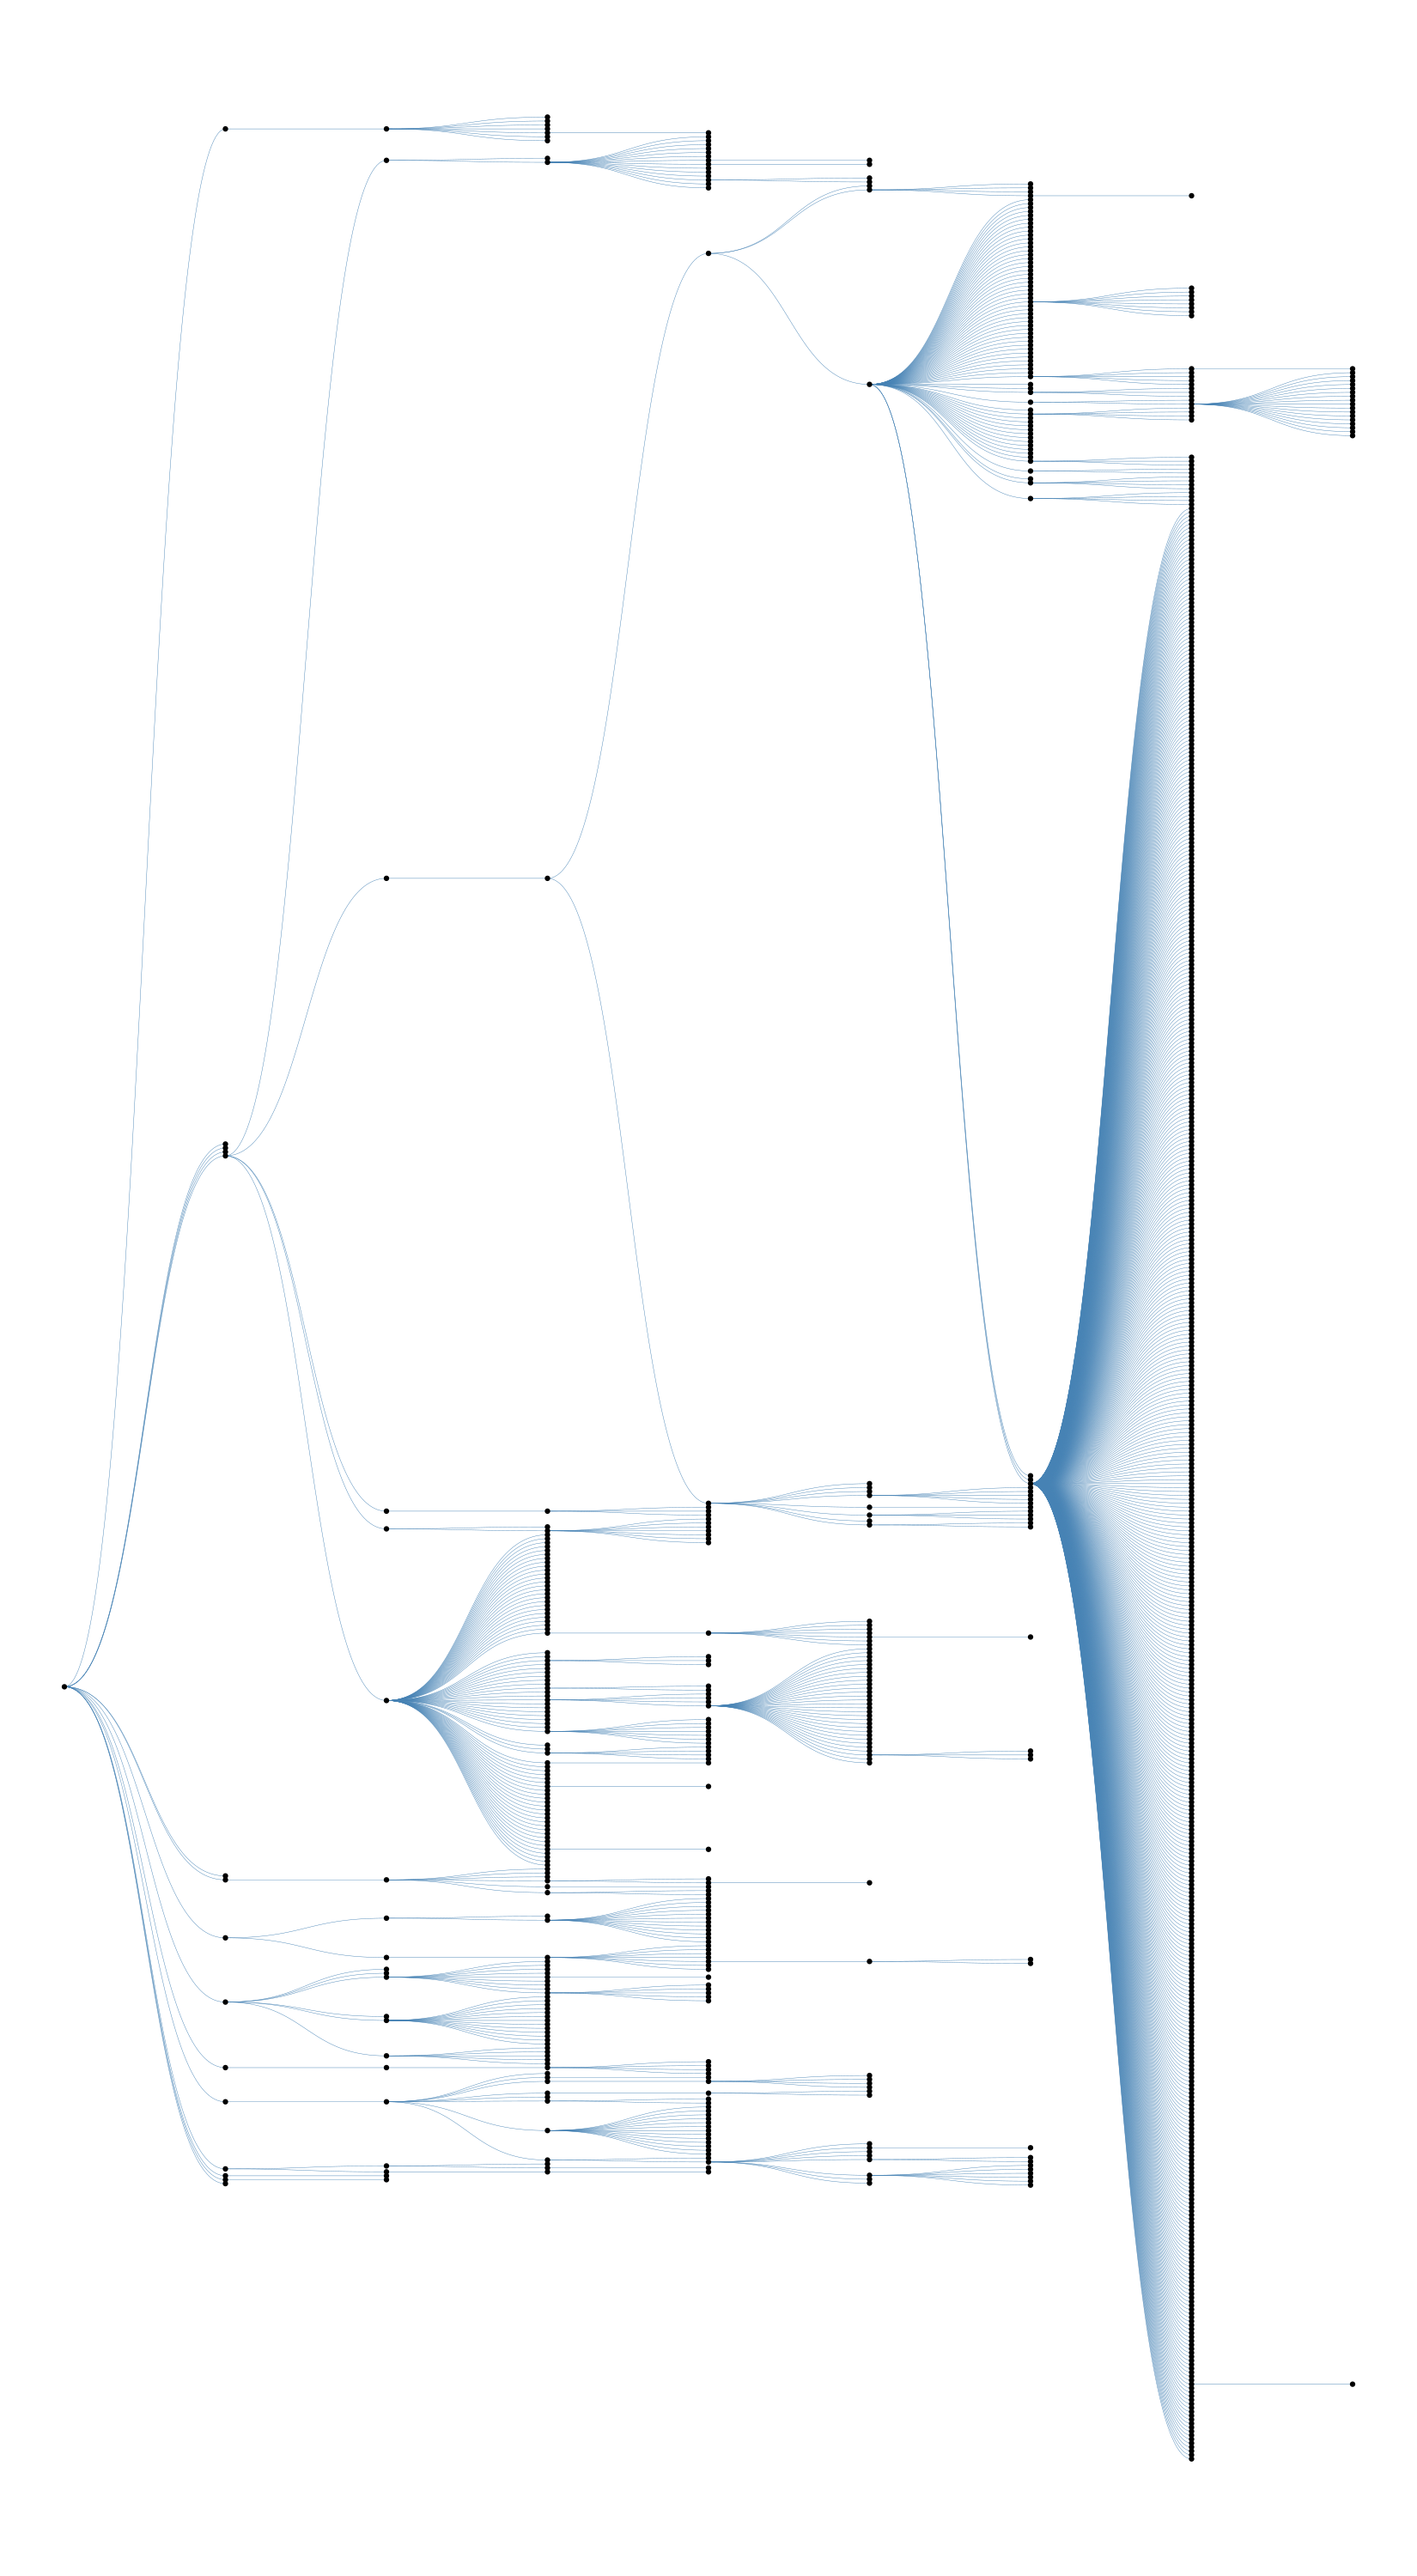
\includegraphics[height = \textheight]{fig-dendrogram-1.png}}
		\label{fig:fig-dendrogram-1}
		\vspace{0.1 in}
	\end{center}
\end{figure}
\setstretch{2.0}

\clearpage
\setstretch{1.0}
\newpage
\begin{figure}[h]
	\begin{center}
		\caption{Nested Structure of the Gulf War (1991)}
		{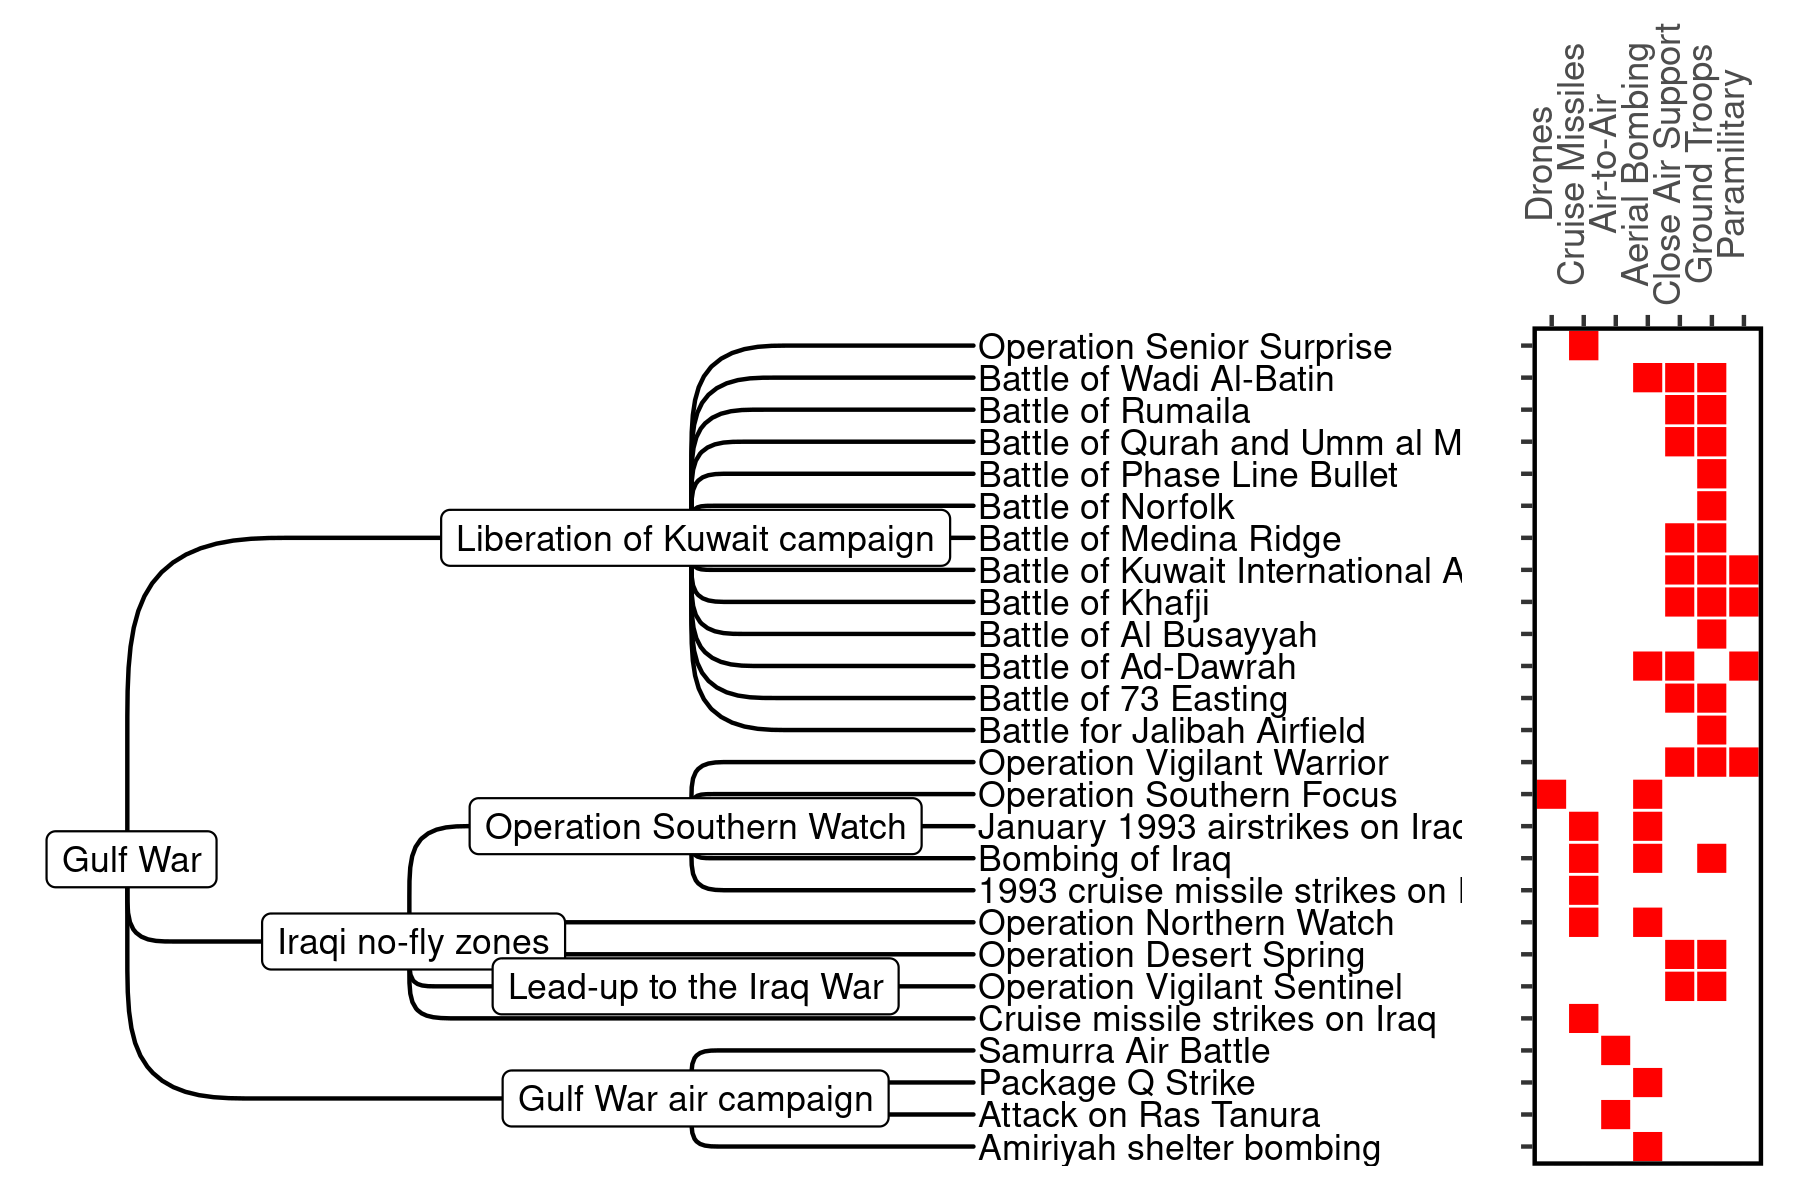
\includegraphics[width = \textwidth]{fig-nested-1.png}}
		\label{fig:fig-nested-1}
		\vspace{0.1 in}
	\end{center}
\end{figure}
\setstretch{2.0}

\clearpage
\setstretch{1.0}
\newpage
\begin{figure}[h]
	\begin{center}
		\caption{Locations of US Military Interventions (1989-2021)}
		{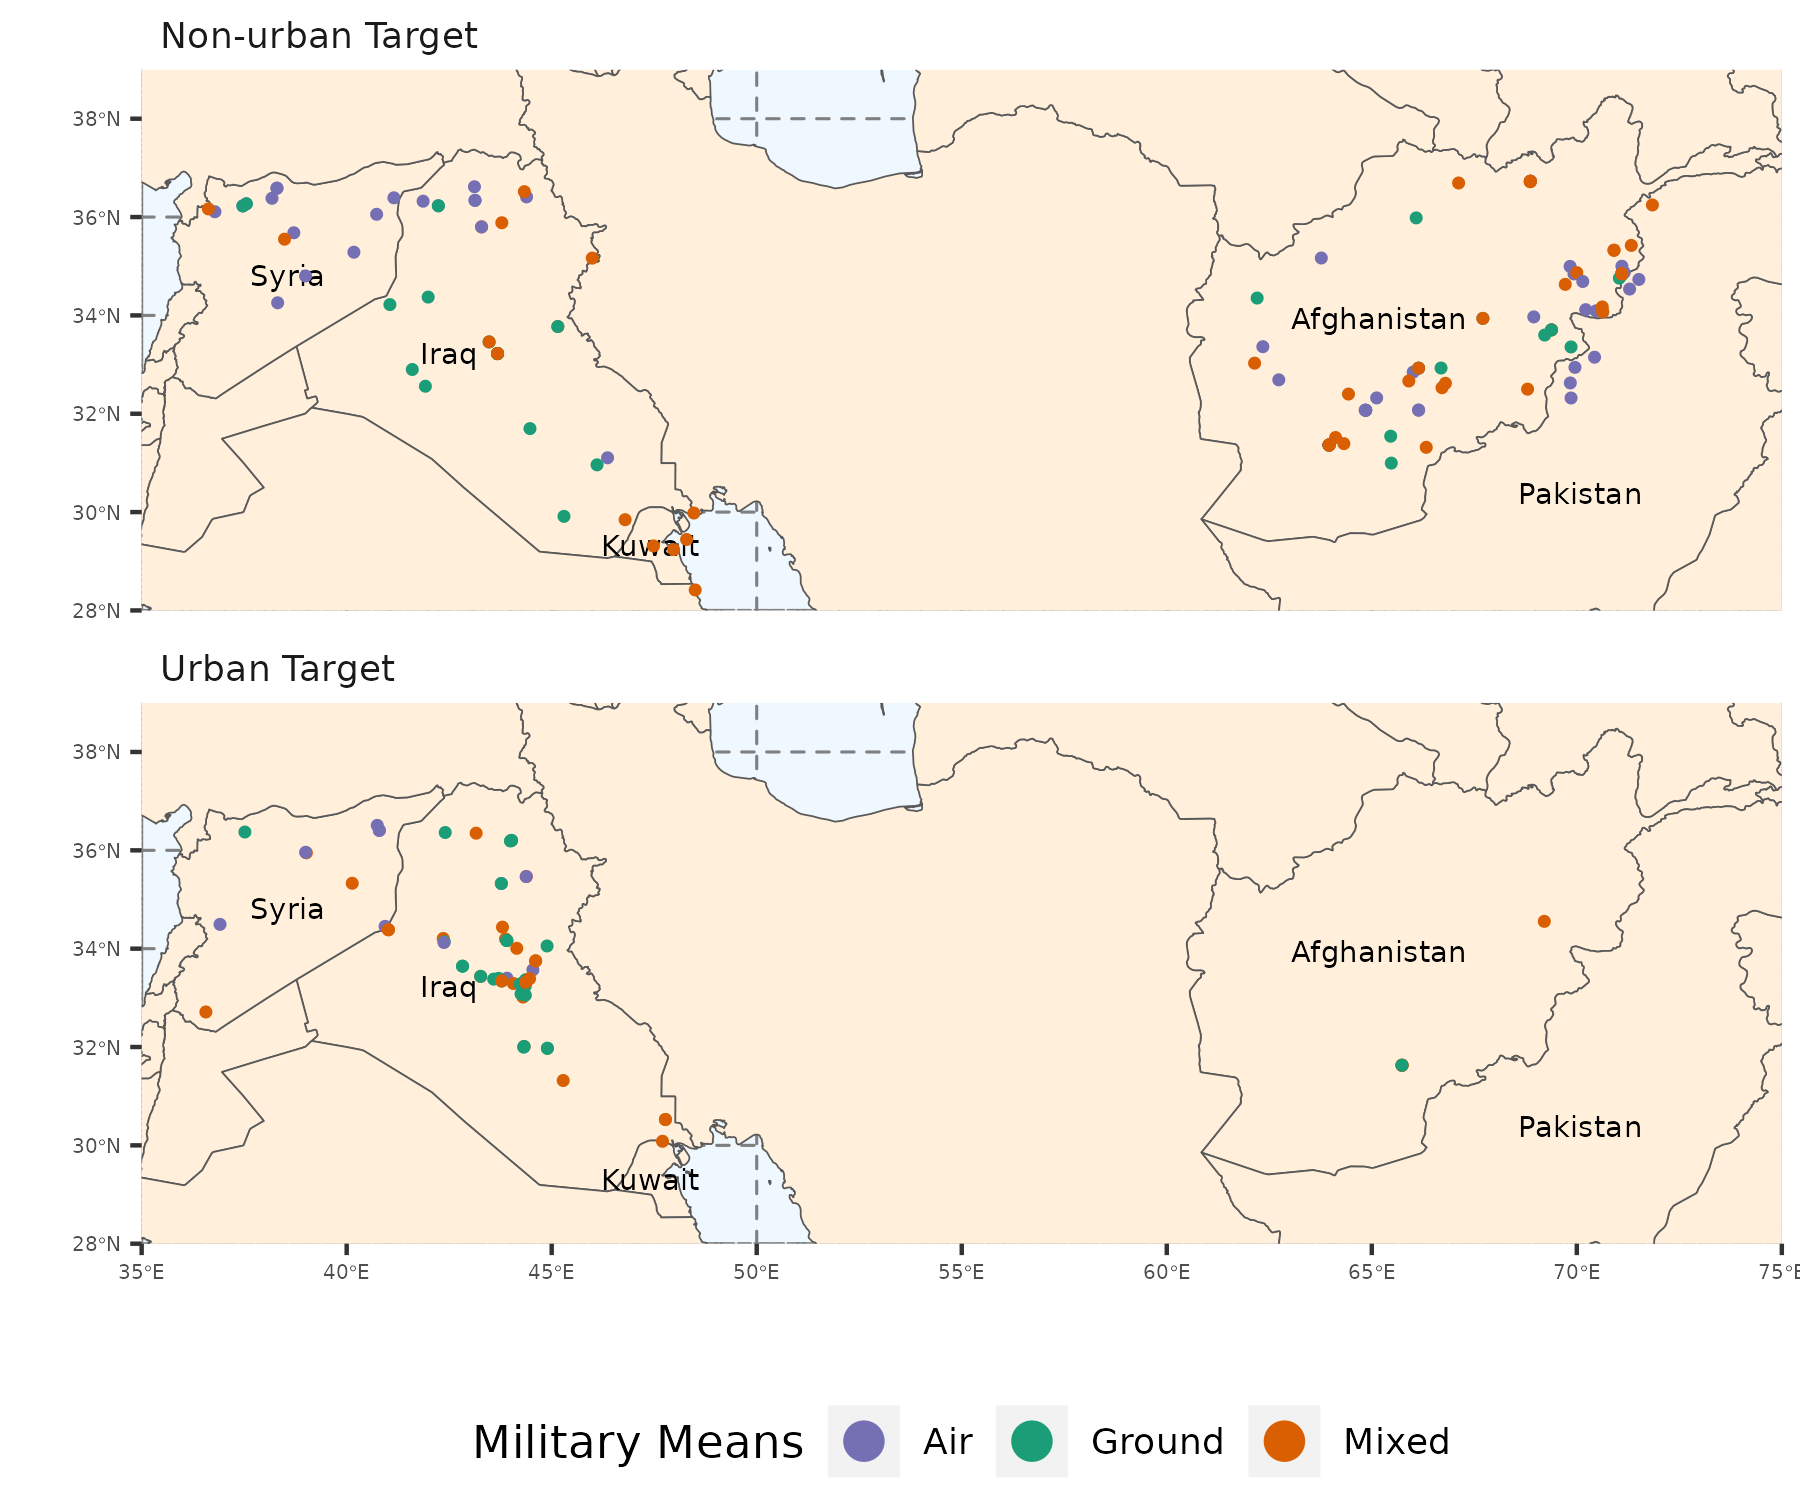
\includegraphics[width = \textwidth]{fig-map-1.png}}
		\label{fig:fig-map-1}
		\vspace{0.1 in}
	\end{center}
\end{figure}
\setstretch{2.0}

\clearpage
\setstretch{1.0}
\newpage
\begin{figure}[h]
	\begin{center}
		\caption{Social Network Plots of Select Conflicts}
		{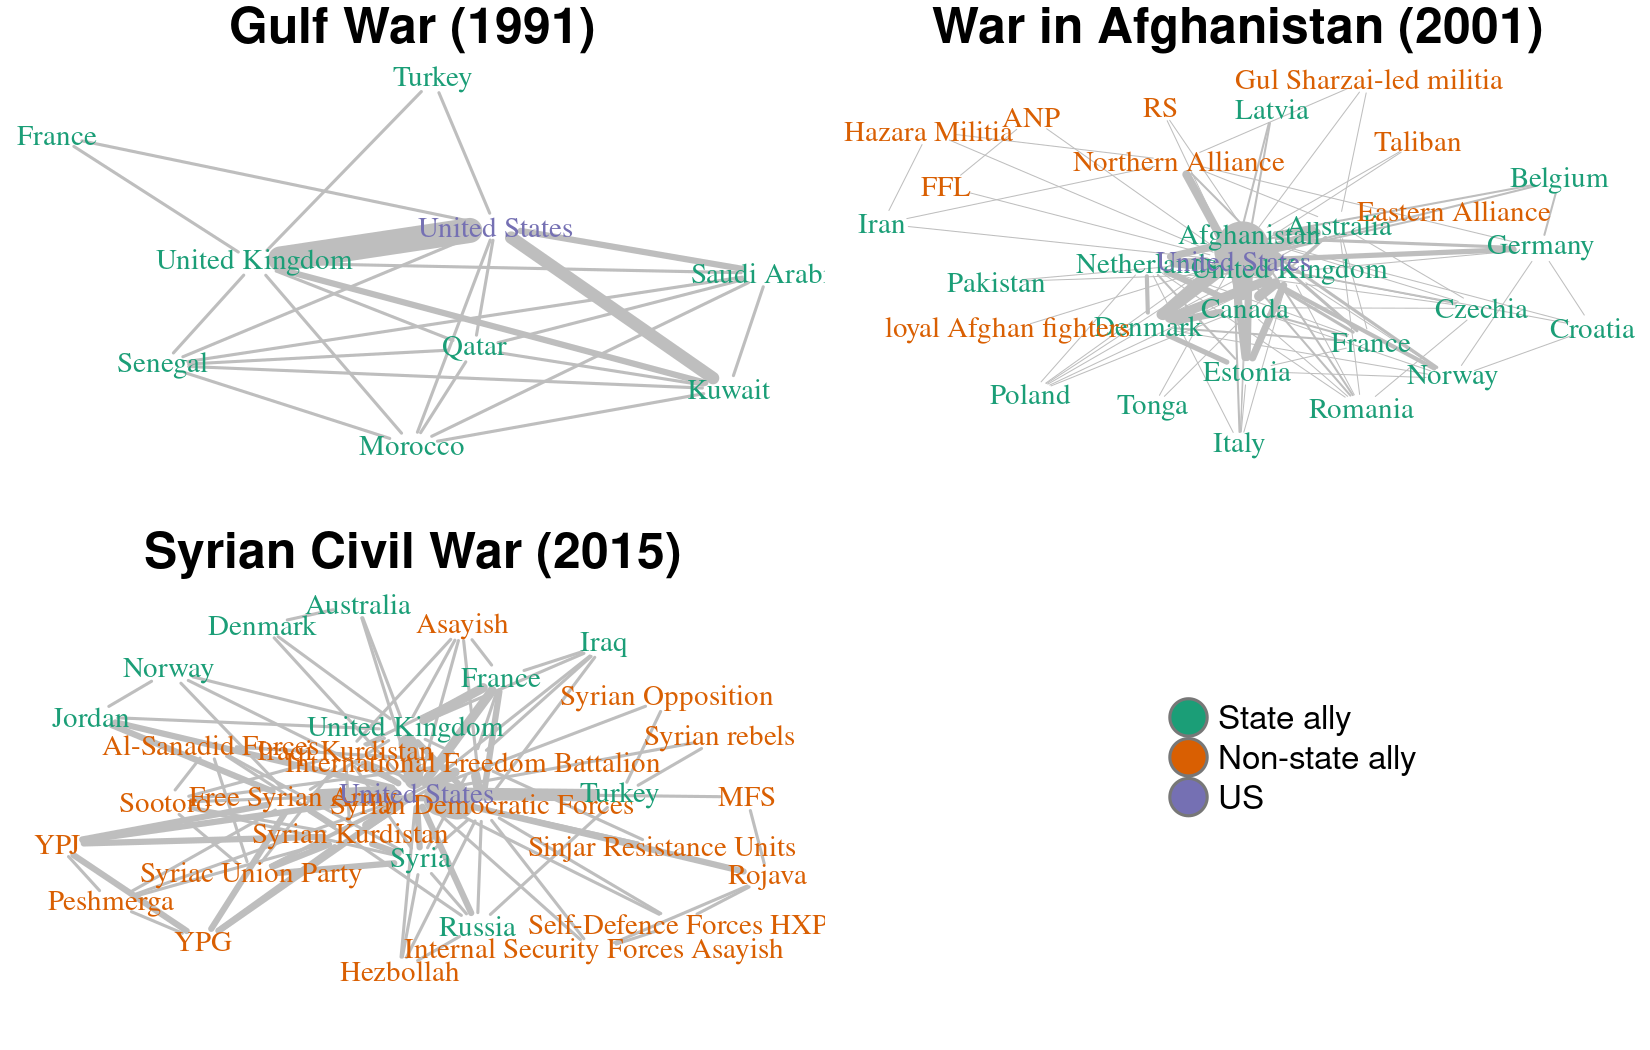
\includegraphics[width = \textwidth]{fig-actors-1.png}}
		\label{fig:fig-actors-1}
		\vspace{0.1 in}
	\end{center}
\end{figure}
\setstretch{2.0}

\clearpage

\newpage

\bibliography{MONSTr.bib}

\end{document}